%------------------------------------------------------
%Author             : Daniel Schembri, Jonathan Schwarz
%University         : Pforzheim University
%Date of last edit  : Wed, 03 Sep 2014 14:12:16 +0200
%Filename           : multithreading_with_posix_pthreads.tex
%------------------------------------------------------

\documentclass[10pt,a4paper,DIV=11]{scrreprt}

%British English
\usepackage[ngerman, UKenglish]{babel}
%utf8
\usepackage[utf8]{inputenc}

%Multicolumn lists
\usepackage{multicol}

%pseudo-code
\usepackage[boxruled,vlined]{algorithm2e}

%for source code listings
\usepackage{listings}

\usepackage[table]{xcolor}

%tikz
\usepackage{tikz}
\usetikzlibrary{arrows,positioning,fit}

%plots
\usepackage{pgfplots}
\usetikzlibrary{calc}
%\usepackage{amsmath}

%blocks - used by tikz-uml, included before
\pgfdeclarelayer{background}
\pgfdeclarelayer{foreground}
\pgfsetlayers{background,main,foreground}

%<,> in tikz-uml
\usepackage[T1]{fontenc}
\usepackage{tikz-uml}

%subfigure
\usepackage{graphicx}
%\usepackage{subfigure}
\usepackage{caption}
\usepackage{subcaption}

%prevent figure from floating pictures
\usepackage{float}

%footer & header
\usepackage{fancyhdr}

%push footer down
\usepackage[bottom]{footmisc}

%footer & header
\pagestyle{fancy}
%clean footer & header
\fancyhf{}

%bibtex
\usepackage[square,numbers]{natbib}
\usepackage{gensymb}

%equation
\usepackage[tbtags]{amsmath}
\usepackage{amssymb} 

%table of contents with hyperlinks
%always include as last package
\usepackage{hyperref}


%===========================TITLE PAGE=======================================

%university logo
\titlehead
{
    
\includegraphics[width=0.20\textwidth]{files/hspflogo.pdf}\\

    Pforzheim University\\
    School of Engineering\\
}

\subject{Project work}
	
\title
{
    Simulation and evolutionary training of object collecting agents\\
}

\author
{
    by \textbf{Daniel Schembri} - matriculation number: 310026
}
\date
{
    Summer term 2015 \\
    \today{}
}


\publishers
{
    Examiner: Prof. Dr. Richard Alznauer\\
    Supervisor: Dr. Christoph Ussfeller
}


%=========================================GLOBAL SETTINGS=========================================

%footer &header

%\fancyfoot[L]{\textbf{Multi-Threading mit POSIX-pThreads}}
\fancyhead[R]{Page \thepage}
%\fancyhead[L]{\thechapter}

%chapter number and title
\fancyhead[L]{\nouppercase{\leftmark}}
%line
%\renewcommand{\footrulewidth}{0.5 pt}
\usepackage{lmodern}
\addtokomafont{sectioning}{\rmfamily}
\setlength{\parindent}{0mm}

%colour definitions
\definecolor{dkgreen}{rgb}{0,0.6,0}
\definecolor{gray}{rgb}{0.7,0.7,0.7}
%medium gray
\definecolor{mgray}{gray}{0.80}
%light gray
\definecolor{lgray}{gray}{0.97}

%hyperlink settings
%frame around hyperlinks
\hypersetup
{
    colorlinks = false,
    linkcolor = black,
    hypertexnames = false,
    citecolor = green
}

%listing settings
\lstset
{ 
    language=C++,                
    basicstyle=\footnotesize\ttfamily,           
    numbers=left,
    stepnumber=5,    
    firstnumber=1,
    numberfirstline=true                 
    numberstyle=\color{black},                 
    numbersep=5pt,                 
    backgroundcolor=\color{white},      
    showspaces=false,             
    showstringspaces=false,         
    showtabs=false,                
    frame=single,                   
    rulecolor=\color{black},       
    tabsize=2,                     
    captionpos=b,                   
    breaklines=true,                
    breakatwhitespace=false,       
    title=\lstname,                    
    keywordstyle=\color{blue},          
    commentstyle=\color{dkgreen}, 
    identifierstyle=\color{black},      
    stringstyle=\color{purple},      
    escapeinside={\%*}{*)},      
    morekeywords={*,...},            
    deletekeywords={...}             
}

\setcounter{tocdepth}{4}  %a deeper contentsmenue
%=====================================DOCUMENT START=========================
\begin{document}

\tikzstyle{line}=[draw]
\tikzstyle{arrow}=[draw, -latex] 

%\renewcommand*\contentsname{Content}
%\renewcommand*\listtablename{Tables}
%\renewcommand*\listfigurename{Figures}
%\renewcommand*\bibname{Literature references}

\maketitle
\thispagestyle{empty}
\newpage
{\large\tableofcontents}




\begin{abstract} 

\huge{\textbf{Erklärung}} \\

\normalsize
Ich versichere, die beiliegende Projektarbeit selbständig verfasst, keine anderen als die angegebenen Quellen und Hilfsmittel benutzt sowie alle wörtlich oder sinngemäß übernommenen Stellen in der Arbeit gekennzeichnet zu haben. \\ \\ \\ \\

\selectlanguage{ngerman}
Kraichtal, den \today{} \hspace{8cm} Daniel Schembri
\selectlanguage{UKenglish}
\end{abstract}


\begin{abstract} 
\huge{\textbf{Abstract}} \\

\normalsize

This document was created for the project work at Pforzheim university in the course: Master of Science in Embedded Systems. 
This projectwork describes the development of a simulation environment for object collecting agents. The agents can base on a simple script or have a neural network that can be trained supervised or evolved by evolutionary algorithms.

The simulator was written in C++ using the 2D physics-engine Box2D by Erin Catto and using the OpenGl-frameworks GLUT, respectively Freeglut for accelerating the displaying of the simulation and GLUI for the graphical user interface. 

The neural network framework is written by Jonathan Schwarz and detaily described in his projectwork ' A comparison of neural network types and learning techniques with an application in artificial life'. \\ \\ \\ \\ \\ \\ \\ \\

\huge{\textbf{Zusammenfassung}} \\

\normalsize

Dieser Projektbericht wurde im Rahmen der Projektarbeit des Studienganges Master of Science in Embedded Systems der Hochschule Pforzheim angefertigt. 

Diese Projektarbeit beschreibt die Entwicklung eines Simulators für virtuelle Agenten, die Objekte in einer 2-dimensionalen Umgebung sammeln. 

Der Simulator wurde in C++ entwickelt. Die Physics-engine Box2D von Erin Catto wird verwendet. Ebenso die OpenGL-Frameworks GLUT bzw. Freeglut zur beschleunigten Darstellung der Simulation und GLUI für die Graphische Benutzer Schnittstelle. 

Das Framework der neuronalen Netze wurde von Jonathan Schwarz entwickelt und wird in seinem Projektbericht 'A comparison of neural network types and learning techniques with an application in artificial life' näher beschrieben.
	
	
\end{abstract}



\chapter{Introduction}
This document was created at Pforzheim University in the course Master of Science in Embedded Systems.
It was part of the project work.

\section{Document structure}
The first chapters explain the basic concepts of software agents, artificial neural networks and evolutionary algorithms.
The following chapters introduce the used libraries and tools.

The main part describes the implementation of the simulator and the theoretical considerations. The last part concludes with the simulation results and a further view of the discussed topic.

\section{Motivation}
The classical method to solve a task mostly is to use a detailed prior knowledge. If this knowledge isn't sufficient it has to be acquired hard. The development of this solution therefore can be difficult, time-consuming and expensive.
This circumstances cause an interest in solving tasks in an universal way. Creatures seems to solve problems easily by the abilities they received by evolution. This motivated researcher to apply this mechanisms in computer science. Thanks to the computing power of today evolution can be used in an abstract way to cultivate solutions and handle optimization problems.

The concept of software agents is one model of artificial intelligence. It's an abstract view of an intelligent system that perceives its environment and acts self-sufficiently.

Artificial neural networks are a concept to approximate target functions. These networks can be used for tasks with just partitial knowledge.
They work well for finding patterns for example.

In this projectwork the main interest lies in agents, artificial neural networks and evolutionary training of these networks.
The motivation is to create a suitable simulation environment and to compare different evolutionary algorithms.



%Today there is no exact definition of what intelligence is. In general there are certain categories focusing different points of view to describe it.


%Artificial intelligence has four branches of research: \\

%\fbox{
%	\begin{minipage}{15cm}
%		\begin{multicols}{2}
%			\begin{itemize}
%				\item \textbf{Knowledge-based systems}
%				\item \textbf{Robotics}
%				\item \textbf{Pattern recognition}
%				\item \textbf{Pattern prediction}
%			\end{itemize}
%		\end{multicols}
%	\end{minipage}
%}    \\

\section{Project task}
The task of this project work is to develop a simulator to let agents collect objects in a 2-dimensional world. As follows a sketch of the main concept: \\

\begin{center}
	\begin{figure}[H]
		\centering
		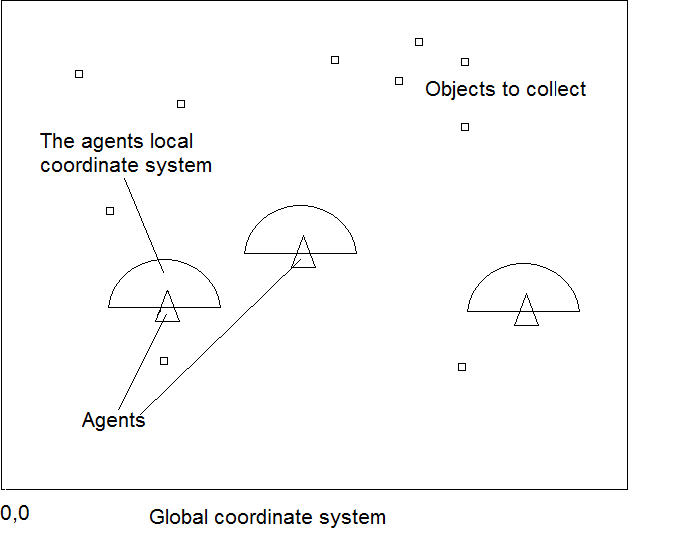
\includegraphics[width=0.7\textwidth,scale=1.0]{files/main-concept.png}  
		\caption{A sketch of the main concept}
		\label{fig:concept-main-intro}
	\end{figure}
\end{center}

The agents and the objects they have to collect are spawned randomly. An agent has to collect as much objects as possible in a given time. Every agent has a sensor, represented by the semicircle in the sketch, to get the distance vector of an object.
The object is just detected if it is in range of the sensor. For simplicity just the position of the nearest object is given, if more objects are in range of the sensor. Based on this input data the agent has two possibilities to act: it can rotate left or right and it can drive forward. Therefore the agents output has two parameters, defining the rotation- direction and speed and the velocity.
To choose the parameters the agent has a logic, processing the input.

This logic is realized  by a neural network that is trained supervised or evolved with special algorithms derived from evolution theory.
The simulator has to simulate a realistic environment. Therefore a physics engine is used.
The simulation has to be rated and the collected data displayed. The simulator uses the neural network framework developed by Jonathan Schwarz.
Artificial neural networks are evolved in this project work to see if they can solve the task satisfactionally.
The concept of software agents is used as a frame to get an abstract view of the used algorithms. \\


%In this project neural networks of the second generation are used, because the main interest lies in finding a good mathematical solution.


\chapter{The concept of agents}
An agent is a program that interacts self-sufficently depending on its actual state. In general, it has sensors, a processing logic and actuators. The input data will be processed to behave in the desired way. In the simplest case this could be a table containing the required output to every possible input.

Most agents are found in the world wide web. For example webcrawlers, search-engines and bots are well known.

In this project the concept of software agents is used as a modelling framework to differentiate the agent from the environment.

The following figure shows the general structure of an agent:


\begin{center}
	\begin{figure}[H]
		\centering
		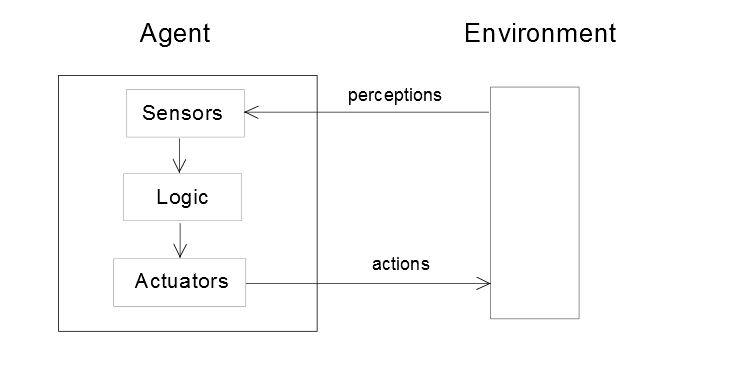
\includegraphics[width=1.0\textwidth,scale=1]{files/agent.png}  
		\caption{General structure of an agent (oriented on \cite{ai} Figure 2.9)} 
		\label{fig:agent}
	\end{figure}
\end{center}

The logic part of an agent can be less or more complex. Just the actual perception can be processed or a specified sequence of perceptions. This could be realised by a simple script for example.
In this project the agents logic is realised as a artificial neural network.

In the following sections the different realisation types of the logic is described in detail.


\section{Rationality \cite{ai}}
An agent creates a sequence of actions. These actions cause a sequence of states in the corresponding environment. Every sequence of states can be rated. The agent is called rational if it can maximize its score, considering its sequence of perceptions and its previous knowledge of the problem. Its important to distinguish rationality and perfection. An agent never will be perfectly solving a problem. It's unrealistic to expect the best possible solution for a problem in partitial observable environments. It can solve the problem as it can be expected by the given perceptions. The agent can't predict random events.

In order to achieve rationality the following topics have to be considered: \\

\fbox{
	\begin{minipage}{15cm}
		\begin{itemize} 
			\item A sufficient previous knowledge of the problem
			\item A good rating of the resulting state sequence of the environment
			\item The perception sequence
			\item The possible actions the agent can execute
		\end{itemize}
	\end{minipage}
}   \\
See also \cite{ai} chapter 2.2.1

\section{Types of agents}
By \cite{ai} agents can be classified in the following categories:
\subsection{Simple reflex agent}


\begin{center}
	\begin{figure}[H]
		\centering
		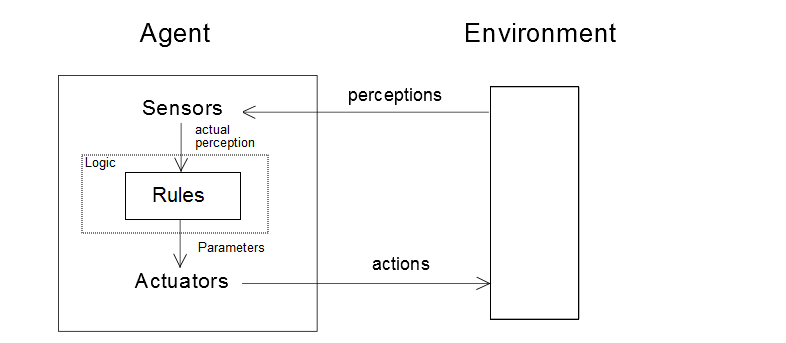
\includegraphics[width=1.0\textwidth,scale=1]{files/Reflexagent.png}  
		\caption{Structure of a simple reflex agent (oriented on \cite{ai} Figure 2.9)} 
		\label{fig:agentr}
	\end{figure}
\end{center}

The simplest type of an agent is the reflex based agent.
This agent only processes the actual perception and act on the base of this actual state. In the simplest case the logic is realised as a lookup table or defined by simple rules. This type of agent can be used for simple tasks. The benefits are a fast implementation and a drastically reduced state space.
The disadvantage lies within the simplicity. This agent has no memory and therefore doesn't include past states in his decisions. If the present state of the environment doesn't provide enough information or it is just partially observable, the agent could not solve the task.
In partially observebale environment there can occur loops of wrong behaviour. This loops can be overcome if a random action can be chosen.
For best functionality of a simple reflex agent the problem-environment should be fully observable.\footnote{See Chapter \ref{sec:env} for an explanaition of the environment}
For more complex tasks using the following described agent-types may be a better solution.
(\cite{ai} chapter 2.4.2)
\subsection{Model-based reflex agent}
The model-based reflex agent expands the simple reflex agent by a memory. It internally creates a model of the world by past sensor data. This model is used to predict future states in the environment.
This can be a moving object or changes in the environment made by the agent itself for example.

Internal states of the agent are used to approximate the state of the environment if changes occur. 
The model is also used to estimate temporaly unobservable parts of the environment.

The model-based reflex agents ability to solve a task reaches its limit, if it has to act in a new environment or other agents acting in the world, too. The internally created model then may not fit anymore.
(\cite{ai} chapter 2.4.3)

\subsection{Goal-based agent}
For some tasks it isn't enough to know the correct action on a specified state at the environment, like reflex-based agents do. It can be important for an agent to know the goal behind those actions. This is necessary for the generalization of a problem. For example: For a given route A To B there can be a description for a sequence of actions the agent has to execute in order to reach the target B. It is more difficult to describe specific rules for getting from one point to another in general, as other routes may differ a lot. It's therefore too complex to describe all rules in detail; hencefore a generalization of this task has to be modelised.

The benefit is an agent that can solve complex tasks. The drawback is a need of more computing time. For real-time tasks this can be an obstacle.
(\cite{ai} chapter 2.4.4)

\subsection{Utility-based agent}
The utility-based agent expands the goal-based agent by the fact, that it can choose between several solutions. Therefore the agent has a rating function to choose the best or at least a good enough solution by several criteria. This rating function can be more complex then computing solutions of the task itself.

The development of such complex agent and corresponding rating algorithms can be difficult and is an own topic of computer science and includes research areas like perception, representation, reasoning and learning.
(\cite{ai} chapter 2.4.5)

\subsection{Learning agent}
The complete development of an agent is difficult and time-consuming. Therefore Alan Turing searched in 1950 for a way to speed up this process.\cite{turing} The concept of the learning agent was created. The learning agent has four components: \\

\fbox{
	\begin{minipage}{15cm}
		\begin{multicols}{2}
			\begin{itemize}
				\item \textbf{Performance element}
				\item \textbf{Learning element}
				\item \textbf{Critic}
				\item \textbf{Problem generator}
			\end{itemize}
		\end{multicols}
	\end{minipage}
}   \\
\\


%\begin{center}
%	\begin{figure}[H]
%		\centering
%		\includegraphics[width=1.0\textwidth,scale=1]{files/Learningagent.png}  
%		\caption{General structure of a learning agent (oriented on \cite{ai} Figure 2.15)} 
%		\label{fig:agentl}
%	\end{figure}
%\end{center}

The \textbf{performance element} is the executive part of the agent. It processes sensor data and makes actions. \\

The \textbf{learning element} is responsible for improvements of the agent. The learning element can contain a decision tree, a neural net, a support vector machine or other learning structures. \\

The \textbf{critic} rates the performance element and tells the learning element how to improve it. \\

A \textbf{problem generator} is used to improve learning by making new experiences. Without the problem generator the agent would work with its best actions, but would never try new actions, that may seem uneffective in the first way, but may prove to be more effective in a long term run. 

It can be important for the agent to gain further knowledge by its perceptions. Therefore the agent has to make some actions to explore the world, if he acts in a unknown environment.
An agent who doesn't learn can most likely not solve a problem if the environment changes.
In nature animals are equipped with reflex actions to survive long enough to learn to adapt to their enviroment. \\


The most important part for improvements is the correlation between the \textbf{performance element} and the \textbf{learning element}.

(\cite{ai} chapter 2.4.6)

\section{The task environment}
\label{sec:env}
In the first case its preferable to define the task completely. In \cite{ai} chapter 2.3 the task environment is defined by four categories: \\

\fbox{
	\begin{minipage}{15cm}
		\begin{multicols}{2}
			\begin{itemize} 
				\item \textbf{Performance}
				\item \textbf{Environment}
				\item \textbf{Actuators}
				\item \textbf{Sensors}
			\end{itemize}
		\end{multicols}
	\end{minipage}
}   \\
\\

The \textbf{performance} is defined by the rating the agent can achieve. The performance measure is done by metrics the developer has to choose before creating agents. Metrics can for example be how good an agent solves the problem, how fast it solves it, how efficient it uses ressources, etc. It is possible to rate the agent by multiple criteria. \\

The \textbf{environment} is the frame an agent solves a task within.
If the sensors allow the agent to get the information of the whole environment, the environment is called \textbf{fully observeable}. The agent therefore can get all relevant information for its actions. Otherwise an environment is classified as \textbf{partially observeable}. For example this can be if the sensors are limited or influenced by interferences.
If the agent has no sensors at all, the task environment is called \textbf{unobserveable}. Instinctively you would think this kind of agent would be totally useless, but there exist succesful algorithms to solve problems. For example a vacuuming robot can clean a room effectively. It therefore uses stochastic algorithms. In factories this is used effectively to turn objects on an assembly line. The benefit is less costs in sensors. \\

It can also be necessary to know if the environment is a \textbf{single-} or \textbf{multiagent}-based one. Multiple agents can \textbf{cooperate} or \textbf{compete}. \\

The environment is \textbf{deterministic} if all further states are predictable by the current state and there are no random events. Otherwise it is \textbf{stochastic}.
In a stochastic environment there are given probabilities for each possible event. If not it is called \textbf{non-deterministic}.
In reality there can exist deterministic environments with the disadvantage of too much possibilities. An agent can't  compute every possible effect then.
In this case the environment must be handled by the agent as if it were stochastic to get a chance of solving the task. \\

If the action of the agent does only depend on the actual environment state and does not influence future state the environment is called \textbf{episodic}. Otherwise its called
\textbf{sequential}. Chess for example is a sequential environment because every move can bring the game in a win- or lose-situation. \\

A \textbf{static} environment doesn't change. This makes it easier for the agent to solve a task. A \textbf{dynamic} environment on the other hand needs a continuously observation.
It is possible that the environment is static, but the rating of the agent depends on the passed time. \textbf{semidynamic}. An example for a static environment is chess. Playing chess with a clock is semidynamic. \\

The environment can have \textbf{discrete} or \textbf{continous} states. Chess has discrete states, as it is played move by move. It could get a continous character if the time to calculate a move plays a role. Driving a car is in general continously as accelerating and steering have continous units.\\

The environment can be \textbf{known} or \textbf{unknown}. That means that the agent has foreknowledge about the environment. This category has nothing to do with observability. \\


\textbf{The actuators} are the components an agent uses to interact with the environment. While developing an agent the types of actuators and, for physical agents, the degrees of freedom\footnote{The degrees of freedom are the amount of independent parameters of a physical system that is necessary to describe the state of this system} may be considered.\\

\textbf{The sensors} are responsible for receiving data of the environment. With appropriate algorithms a better evaluation of sensor data is possible. The advantage can be a noticeable reduction of sensor costs.


\chapter{Artificial neural networks}
Artficial neural networks (ANN) are inspired by their biological equivalents.
They are used in machine learning as an own class of classfiers, next to support vector machines
and other mathematical methods. On the one hand there exist models offering biological plausability to research the
operations in the human brain. On the other hand there exist models whos main focus lies in finding good mathematical solutions for technical tasks.

Artificial neural networks are often seen as a black box: \\

\begin{center}
	\begin{figure}[H]
		\centering
		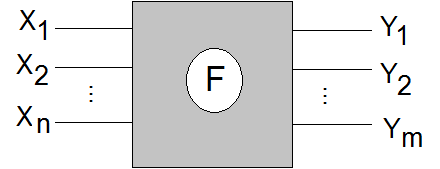
\includegraphics[width=0.5\textwidth,scale=1.0]{files/nn-bb.png}  
		\caption{An ANN as black box \cite{rojas}}
		\label{fig:neuron}
	\end{figure}
\end{center} 
They approximate target functions. For a given input vector $\vec{X}$ an output vector $\vec{Y}$ can be computed.
This happens on the base on a given data set or completely unsupervised.
They map a function as follows\cite{rojas}:

\begin{equation}
	F: R^n \to R^m 
\end{equation} 


In general an ANN has an input layer, containing the inputvector $\vec{X}$ with $n$ components, optional hidden layers and one output layer giving the resultvector $\vec{Y}$ with $m$ components.
All neurons, except the input neurons, have real weighted input connections, an activation function and output values. The input neurons do no computation. They just contain the input data. As follows a neural network:

\def\layersep{2.5cm}
\begin{figure}[H]
\begin{center}
\begin{tikzpicture}[shorten >=1pt,->,draw=black!50, node distance=\layersep]
\tikzstyle{every pin edge}=[<-,shorten <=1pt]
\tikzstyle{neuron}=[circle,fill=black!25,minimum size=17pt,inner sep=0pt]
\tikzstyle{input neuron}=[neuron, fill=green!50];
\tikzstyle{output neuron}=[neuron, fill=red!50];
\tikzstyle{hidden neuron}=[neuron, fill=blue!50];
\tikzstyle{annot} = [text width=4em, text centered]

% Draw the input layer nodes
\foreach \name / \y in {1,...,3}
% This is the same as writing \foreach \name / \y in {1/1,2/2,3/3,4/4}
\node[input neuron] (I-\name) at (0,-\y) {$x_\y$};


% Draw the hidden layer nodes
\foreach \name / \y in {1,...,4}
\path[yshift=0.5cm]
node[hidden neuron] (H-\name) at (\layersep,-\y cm) {};

% Draw the output layer node
%\foreach \name / \y in {1,...,2}
\node[output neuron,pin={[pin edge={->}]right:$Y_1$}, right of=H-2] (O-1) {};
\node[output neuron,pin={[pin edge={->}]right:$Y_2$}, right of=H-3] (O-2) {};
% Connect every node in the input layer with every node in the
% hidden layer.
\foreach \source in {1,...,3}
\foreach \dest in {1,...,4}
\path (I-\source) edge (H-\dest);

% Connect every node in the hidden layer with the output layer
\foreach \source in {1,...,4}
	\foreach \dest in {1,...,2}
	\path (H-\source) edge (O-\dest);

% Annotate the layers
\node[annot,above of=H-1, node distance=1.3cm] (hl) { Hidden layers};
\node[annot,below of=hl, node distance=0.6cm] (h2) {(optional)};
\node[annot,above of=I-1, node distance=1.3cm] {Input layer};
\node[annot,above of=O-1, node distance=1.8cm] {Output layer};

\end{tikzpicture}
	\caption{The general structure of an artificial neural network}
	\label{fig:general-ann}
\end{center}
\end{figure}


\begin{figure}[H]
	\begin{center}
		\begin{tikzpicture}[shorten >=1pt,->,draw=black!50, node distance=\layersep]
		\tikzstyle{every pin edge}=[<-,shorten <=1pt]
		\tikzstyle{neuron}=[circle,fill=black!25,minimum size=17pt,inner sep=0pt]
		\tikzstyle{input neuron}=[neuron, fill=green!50];
		\tikzstyle{output neuron}=[neuron, fill=red!50];
		\tikzstyle{hidden neuron}=[neuron, fill=blue!50];
		\tikzstyle{annot} = [text width=4em, text centered]
		
		% Draw the input neuron
		\node[input neuron] (I-1) at (0,-1)
		{$x_1$};
		\node[input neuron] (I-2) at (0,-2)	
		{$x_2$};
		\node[input neuron] (I-3) at (0,-3)
		{$x_3$};
		% Draw the hidden layer nodes
		\foreach \name / \y in {1,...,1}
		\path[yshift=0.5cm]
		node[hidden neuron] (H-\name) at (\layersep,-2.4cm) {$H_1$};
		% Connect every node in the input layer with every node in the hidden layer.
		\path (I-1) edge node[above]{$w_{11}$} (H-1);	
		\path (I-2) edge node[above]{$w_{12}$} (H-1);
		\path (I-3) edge node[above]{$w_{13}$} (H-1);					
		\draw[->] (H-1) -- (4.5,-1.9cm) node[above]{};
		\draw[->] (H-1) -- (4.5,-1.9cm)
		node[right] {$f(I)$};
		\end{tikzpicture}
		\caption{The input of an neuron}
		\label{fig:neuron-input}
	\end{center}
\end{figure}

The total neuron input $I$ is the sum of all input values $x_i$ multiplied by their given weights $w_{1i}$. The first index 1 stands for the receiving neuron $H1$:
\begin{figure}[H]
	\begin{center}
		\begin{flalign*}
I = \sum_{i=1}^{n}(x_{i}*w_{1i})
		\end{flalign*}
	\end{center}
	\caption{The total neuron input}
	\label{eq:neuroninputex}
\end{figure}

The output of the neuron is then computed by an activation function $f(I)$. Usually all neurons of an entire layer have the same activation function. Commonly used are tangens hyperbolicus and linear functions:

\begin{figure}[H]
\begin{subfigure}[]{0.5\linewidth}
\begin{tikzpicture}
\begin{axis}[
%	name=plot1,
	xmin=-3, xmax=3,
	ymin=-1.5, ymax=1.5,
	y=1.2cm,x=1cm,
	axis lines=center,
	axis on top=true,
	domain=-2.5:2.5,
	ylabel=$Y$,
	xlabel=$I$,
	]
	
	\addplot [mark=none,draw=black,ultra thick] {\x};
%	\node [right, red] at (axis cs: 1,0.7) {$Y = I$};
\end{axis}
\end{tikzpicture}
\begin{align*}
Y = I
\end{align*}
  \caption*{Linear function (here: identity function)}
  \label{fig:sub1}
\end{subfigure}
\hspace{0.5cm}
\begin{subfigure}[]{0.5\linewidth}
\begin{tikzpicture}
\begin{axis}[
%name=plot2, at=(plot1.right of south east),
xmin=-3, xmax=3,
ymin=-1.5, ymax=1.5,
y=1.2cm,x=1cm,
axis lines=center,
axis on top=true,
domain=-2.5:2.5,
ylabel=$Y$,
xlabel=$I$,
]
\addplot [mark=none,draw=black,ultra thick] {tanh(\x)};
%\node [right, red] at (axis cs: 1,0.7) {$Y = \tanh(I)$};

%% Add the asymptotes
%\draw [blue, dotted, thick] (axis cs:-2.5,-1)-- (axis cs:0,-1);
%\draw [blue, dotted, thick] (axis cs:+2.5,+1)-- (axis cs:0,+1);
\end{axis}
\end{tikzpicture}
  \begin{align*}
  Y = \tanh{(I)}
  \end{align*}
  \caption*{Tangens hyperbolicus}
  \label{fig:sub2}
\end{subfigure}
  \caption{Activation functions}
\end{figure}

Activation functions can have a threshold $S$. The neurons output is zero if $I<S$:

\begin{figure}[H]
\begin{subfigure}[]{0.5\linewidth}
	\begin{tikzpicture}
	\begin{axis}[
	%name=plot2, at=(plot1.right of south east),
	xmin=-3, xmax=3,
	ymin=-1.5, ymax=1.5,
	y=1.2cm,x=1cm,
	axis lines=center,
	axis on top=true,
	domain=-2.5:2.5,
	ylabel=$Y$,
	xlabel=$I$,
	]
	\addplot[domain=-3:0,mark=none,draw=black,ultra thick] {0};
	
	\addplot[domain=0:3,mark=none,draw=black,ultra thick] {abs(\x))};
	\end{axis}
	\end{tikzpicture}
	\begin{align*}
	&S = 0 \\
	&Y =
	\begin{cases}
	I       & \quad \text{if } I  \geq S \\
	0  & \quad \text{otherwise}\\
	\end{cases}
	\end{align*}
	\caption*{Identity function with threshold $S$}
	\label{fig:sub3}
\end{subfigure}
\hspace{0.5cm}
\begin{subfigure}[]{0.5\linewidth}
	\begin{tikzpicture}
	\begin{axis}[
	%name=plot2, at=(plot1.right of south east),
	xmin=-3, xmax=3,
	ymin=-1.5, ymax=1.5,
	y=1.2cm,x=1cm,
	axis lines=center,
	axis on top=true,
	domain=-2.5:2.5,
	ylabel=$Y$,
	xlabel=$I$,
	]
	
	\addplot[domain=-3:0.5,mark=none,draw=black,ultra thick] {0};
	
	\addplot[domain=0.5:3,mark=none,draw=black,ultra thick] {1};
	\end{axis}
	\end{tikzpicture}
	\begin{align*}
	&S = 0.5 \\
	&Y =
	\begin{cases}
	1       & \quad \text{if } I  \geq S \\
	0  & \quad \text{otherwise}\\
	\end{cases}
	\end{align*}
	\caption*{Binary function with threshold $S$}
	\label{fig:sub4}
\end{subfigure}
  \caption{Activation functions with threshold}
\end{figure}

It computes this input by an activation function that has to be defined. Usually an entire layer of neurons has the same activation function. It follows commonly used activation functions:
\begin{figure}[H]
	\begin{center}
		\begin{equation}
		f(I)=
		\end{equation}
		\caption{The activation fucntion}
		\label{eq:transferfunction}
	\end{center}
\end{figure} 

 
 It follows an example of the computation of a neural net. Assume there are 3 input neurons and 1 output neuron:

 

\begin{figure}[H]
	\begin{center}
		\begin{tikzpicture}[shorten >=1pt,->,draw=black!50, node distance=\layersep]
		\tikzstyle{every pin edge}=[<-,shorten <=1pt]
		\tikzstyle{neuron}=[circle,fill=black!25,minimum size=17pt,inner sep=0pt]
		\tikzstyle{input neuron}=[neuron, fill=green!50];
		\tikzstyle{output neuron}=[neuron, fill=red!50];
		\tikzstyle{hidden neuron}=[neuron, fill=blue!50];
		\tikzstyle{annot} = [text width=4em, text centered]
		
		% Draw the input neuron
		\node[input neuron] (I-1) at (0,-1)
		{$3$};
		\node[input neuron] (I-2) at (0,-2)	
		{$-1$};
		\node[input neuron] (I-3) at (0,-3)
		 {$0$};
 	%	\node[input neuron] (I-4) at (0,-4) {$2$};
		% Draw the hidden layer nodes
		\foreach \name / \y in {1,...,1}
		\path[yshift=0.5cm]
		node[output neuron] (H-\name) at (\layersep,-2.4cm) {$11$};
		% Connect every node in the input layer with every node in the hidden layer.
		\path (I-1) edge node[above]{4} (H-1);	
		\path (I-2) edge node[above]{1} (H-1);
		\path (I-3) edge node[above]{2} (H-1);	
%		\path (I-4) edge node[above]{-1} (H-1);				
		\end{tikzpicture}
		\caption{The input of an neuron}
		\label{fig:neuron-input-example}
	\end{center}
\end{figure}

 The activation function of this output neuron is defined by the identity function with a threshold: 
 \begin{equation}
 f(I) =
 \begin{cases}
 Z       & \quad \text{if } neuroninput  \geq S \\
 0  & \quad \text{otherwise}\\
 \end{cases}
 \end{equation}
 


In this example the output neuron gets an total input of:
\begin{figure}[H]
	\begin{center}
		\begin{flalign*}
		&x_1=3,\quad x_2=-1,\quad x_3=0\\
		&w_{11}=4,\quad w_{12}=1,\quad w_{13}=2\\
		&neuroninput = \sum_{i=1}^{3}(x_{i}*w_{1i}) = (3*4) + (-1*1) + (0*2) = 11
		\end{flalign*}
	\end{center}
	\caption{The total neuron input}
	\label{eq:neuroninputex}
\end{figure}

It computes this input by its threshold function
\begin{figure}[H]
	\begin{center}
		\begin{equation}
		f(neuroninput)=\tanh{(neuroninput)}
		\end{equation}
		\caption{The activation fucntion}
		\label{eq:transferfunction}
	\end{center}
\end{figure} 



\section{Neuron- and network types}
In this section the different neuron- and networktypes are described by a chronological view.
\subsection{The model of McCulloch and Pitts}
\label{sec:pitts}
The first mathematical model of a neuron was the McCulloch-Pitts-neuron,
developed by Warren McCulloch and Walter Pitts in 1943.\cite{NEURONMATH}
They wanted to realise a simple, realistic neuron-modell of the operations in the human brain and find out if the brain could compute turing computable functions.
McCulloch-Pitts-neuron has binary inputs and one binary output.
A real threshold has to be defined for each neuron, which reached, let the neuron fire\footnote{In biology the word 'fire' means that the neuron puts out a signal} one or otherwise zero as output.
Its possible to add absolute suppressing inputs. If one of these has the value one, the neuron gives out zero, no matter of other inputs.
Its possible to use relative suppressing inputs instead. For each relative suppressing input the threshold of the neuron is then incremented.
\footnote{In \cite{rojas} chapter 2.4.2 it's shown that Mcculloch-Pitts-networks with absolute suppressing inputs can be replaced by networks with relative suppressing inputs and vice versa. The topologies may differ}
In contrast to the general ANN-model, seen in figure \ref{fig:general-ann} this neuron model has no weights.


Neural networks of this type of neuron can just learn by changing the threshold and the topology of the network. This causes an unnecessary workload due to its high effort in implementation.

At the following a figure of a single neuron is shown:

\begin{figure}[H]  % [H] erzwingt Position an der Stelle im Text
	\centering
	\begin{tikzpicture}
	\node [align=center] (dummy1) at (-0.25,3.5) {$x_{1}$}; 
	\node [align=center] (dummy2) at (-0.25,2.5) {$x_{n}$}; 
	\node [draw=black, fill=white, align=center, circle] (f1) at (1,3) {f}; 		
	\node [align=center] (dummy3) at (3,3) {f($x_{1}$,..,$x_{n}$)}; 
	\draw[arrow]	(dummy1) -- (f1);
	\draw[arrow]	(dummy2) -- (f1);
	\draw[arrow]	(f1) -- (dummy3);
	\draw[dotted] (dummy1) -- (dummy2);
	
	\end{tikzpicture}
	\caption{A McCulloch-Pitts-neuron}
	\label{fig:pitts1}
\end{figure}

In general a neuron can be considered as a function.
The neuron has n inputs and 1 output that can be connected to multiple neurons. It has an activation function that puts out the value one if the threshold $S$ is reached. \\

The overall input is computed by:

\begin{equation}
neuroninput = \sum_{i=1}^{n} x_{i} \quad  x \in \{0, 1\}
\end{equation}

$x_{n}$ are the binary inputs. \\

The output Y is:


\[ Y =
\begin{cases}
1       & \quad \text{if } neuroninput  \geq S \\
0  & \quad \text{otherwise}\\
\end{cases}
\]




%Source Rochas

A function composition:

\begin{figure}[H]
	\centering
	\begin{tikzpicture}
	\node [align=center] (dummy1) at (-0.25,3.5) {$x_{1}$}; 
	\node [align=center] (dummy2) at (-0.25,2.5) {$x_{n}$}; 
	\node [draw=black, fill=white, align=center, circle] (f1) at (1,3) {f}; 		
	\node [draw=black, fill=white, align=center, circle] (g1) at (2.5,3) {g}; 
	\node [align=center] (dummy3) at (4.5,3) {g(f($x_{1}$,..,$x_{n}$)}; 
	\draw[arrow]	(dummy1) -- (f1);
	\draw[arrow]	(dummy2) -- (f1);
	\draw[arrow]	(f1) -- (g1);
	\draw[arrow]	(g1) -- (dummy3);
	\draw[dotted] (dummy1) -- (dummy2);
	
	\end{tikzpicture}
	\caption{Function composition of two McCulloch-Pitts-neurons}
	\label{fig:pitts2}
\end{figure}

The function composition is a concatenation of multiple neurons. \\

A recursive neuron:

\begin{figure}[H]
	\centering
	\begin{tikzpicture}
	\node [align=center] (dummy1) at (-0.25,3) {$x_{t}$}; 
	\node [draw=black, fill=white, align=center, circle] (f1) at (1,3) {f}; 		
	\node [align=center] (dummy2) at (4,3) {f($x_{t}$,f($x_{t-1}$,f($x_{t-2}$,...)))}; 
	\draw[arrow]	(dummy1) -- (f1);
	\draw[arrow]	(f1) -- (dummy2);
	\draw[arrow] (1.35,3) .. controls (1.3,2.15) and (0.6,2.2) .. (0.70, 3);
	\end{tikzpicture}
	\caption{Recursive McCulloch-Pitts-neuron}
	\label{fig:pitts3}
\end{figure}

The output is given after a defined timestep $t$. $t$ represents the amount of cycles a recursive neural net computes before the output is used. A recursive computation of a neuron can be stopped after any  timestep and the output can be used. A recursive connection behaves like a memory that contains the amount of $t$ post states.

\paragraph{Applications}
The McCulloch-Pitts-neuron is biologically not plausible, because learning
can just happen by changing the threshold and the network topology. This needs complex algorithms.
But this neuron type can realise AND-, OR- and NOT-Gates.
Therefore a network of neurons can realise every boolean logic and it is used in electrical engineering, because of realising logic gates efficently in contrast to classical gates. You can simulate finite state machines, too.
You may think if its better to have real or at least integer values to transmit more information instead of just binary signals. However this depends on the application type. Binary values are easier to realize, both in electrical and biological systems and mcculloch-pitts-networks are equivalent to other kind of networks with more signalstates. Though you get a more complex network topology, if you use binary neurons.

It was the first mathematical model of artifical neural networks.


\subsection{Perceptron}
The classical perceptron was published by Frank Rosenblatt in 1958.
It has just an input- and an outputlayer with binary values. In contrast to the McCulloch-Pitts-neuron
the perceptron has additionally real weights. The advantage is that learning-algorithms just have to change the weights instead of the topology or the threshold. It's possible to define positive (stimulation), negative (supression) and zero (neutral) weights.

\subsubsection*{Linear seperability (TODO)}
One main task of neural networks is to classify data. The net is therefore used as a seperator.
The classical perceptron can seperate linear datasets. 


\begin{figure}[H]
	\centering
	%	\subfigure[]
	%	{
	\begin{tabular}{|c|c|c|}
		\hline
		x1 & x2 & f(x1, x2)\\
		\hline
		0 & 0 & 0 \\
		\hline
		0 & 1 & 1 \\
		\hline
		1 & 0 & 1 \\
		\hline
		1 & 1 & 1 \\
		\hline
	\end{tabular}
	%}
	\caption{OR-Function: linear seperable}
	\label{fig:linsep1}
\end{figure}

\begin{figure}[H]
	\begin{center}
		\begin{tikzpicture}
		\tikzstyle{point}=[circle,fill=black!255,minimum size=7pt,inner sep=0pt]
		
		\draw[->] (-0.2,0) -- (3,0) node[right] {$x1$};
		\draw[->] (0,-0.2) -- (0,3) node[above] {$x2$};
		\node at (0,-0.5) {0};
		\node at (-0.5,0) {0};
		\node at (-0.5,2.5) {1};
		\node at (2.5,-0.5) {1};
		\draw plot[mark=square*, mark options={fill=white}] (0,0);
		\draw plot[mark=*, mark options={fill=black}] (2.5,0);
		\draw plot[mark=*, mark options={fill=black}] (0,2.5);
		\draw plot[mark=*, mark options={fill=black}] (2.5,2.5);
		\draw (0,1.3) -- (1.3,0); 
		%legend
		\draw plot[mark=square*, mark options={fill=white}]
		(0,-1.5);
		\node at (0.8,-1.5) {False};
		\draw plot[mark=*, mark options={fill=black}]
		(0,-1);
		\node at (0.8,-1) {True};
		
		\end{tikzpicture}
	\end{center}
	\caption{Or-Function: separation function}
	\label{fig:sepplot1}	
\end{figure}


\begin{figure}[H]
	\centering
	%	\subfigure[]
	%	{
	\begin{tabular}{|c|c|c|}
		\hline
		x1 & x2 & f(x1, x2)\\
		\hline
		0 & 0 & 0 \\
		\hline
		0 & 1 & 0 \\
		\hline
		1 & 0 & 0 \\
		\hline
		1 & 1 & 1 \\
		\hline
	\end{tabular}
	%}
	\caption{And-Function: linear separable}
	\label{fig:linsep2}
\end{figure}

\begin{figure}[H]
	\begin{center}
	\begin{tikzpicture}
		\tikzstyle{point}=[circle,fill=black!255,minimum size=7pt,inner sep=0pt]
			
		\draw[->] (-0.2,0) -- (3,0) node[right] {$x1$};
		\draw[->] (0,-0.2) -- (0,3) node[above] {$x2$};
		\node at (0,-0.5) {0};
		\node at (-0.5,0) {0};
		\node at (-0.5,2.5) {1};
		\node at (2.5,-0.5) {1};
		\draw plot[mark=square*, mark options={fill=white}] (0,0);
		\draw plot[mark=square*, mark options={fill=white}] (2.5,0);
		\draw plot[mark=square*, mark options={fill=white}] (0,2.5);
		\draw plot[mark=*, mark options={fill=black}] (2.5,2.5);
		\draw (0,2.8) -- (2.8,0); 
		%legend
		\draw plot[mark=square*, mark options={fill=white}]
		(0,-1.5);
		\node at (0.8,-1.5) {False};
		\draw plot[mark=*, mark options={fill=black}]
		(0,-1);
		\node at (0.8,-1) {True};

	\end{tikzpicture}
	\end{center}
	\caption{And-Function: separation function}
	\label{fig:sepplot2}	
\end{figure}

XOR-Problem

\begin{figure}[H]
	\begin{center}
		\begin{tikzpicture}
		\tikzstyle{point}=[circle,fill=black!255,minimum size=7pt,inner sep=0pt]
		
		\draw[->] (-0.2,0) -- (3,0) node[right] {$x1$};
		\draw[->] (0,-0.2) -- (0,3) node[above] {$x2$};
		\node at (0,-0.5) {0};
		\node at (-0.5,0) {0};
		\node at (-0.5,2.5) {1};
		\node at (2.5,-0.5) {1};
		\draw plot[mark=square*, mark options={fill=white}] (0,0);
		\draw plot[mark=*, mark options={fill=black}] (2.5,0);
		\draw plot[mark=*, mark options={fill=black}] (0,2.5);
		\draw plot[mark=square*, mark options={fill=white}] (2.5,2.5);
		\node at (1.5,1.5) {?};
		%\draw (0,2.8) -- (2.8,0); 
		%\draw (0,2.0) -- (2.0,0); 
		%legend
		\draw plot[mark=square*, mark options={fill=white}]
		(0,-1.5);
		\node at (0.8,-1.5) {False};
		\draw plot[mark=*, mark options={fill=black}]
		(0,-1);
		\node at (0.8,-1) {True};
		
		\end{tikzpicture}
	\end{center}
	\caption{XOR: separation function}
	\label{fig:sepplot3}	
\end{figure}

\paragraph{Applications}
The perceptron can be used as pattern associator to assign an input pattern to a class. It can also be used as competitive network. Also linear seperable data can be categorised.
It can be trained with the hebbian- or the delta-learning rule.(see also \eqref{sec:learning})

\begin{center}
	\begin{figure}[H]
		\centering
	%	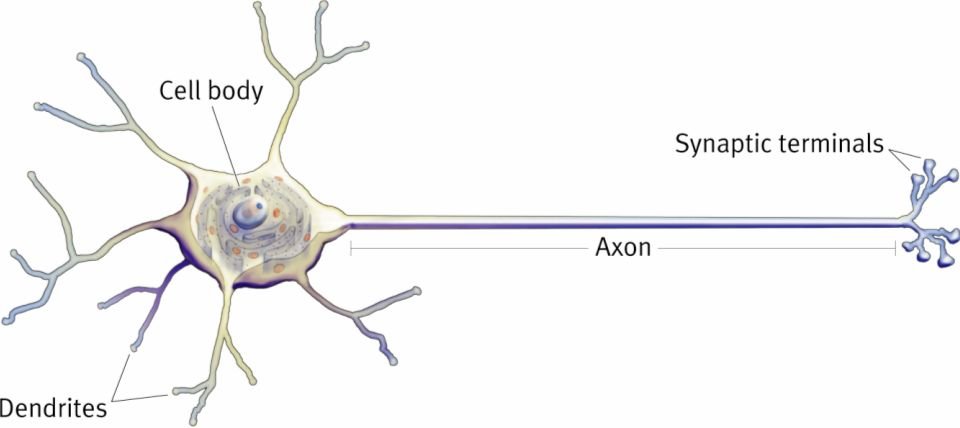
\includegraphics[width=0.8\textwidth,scale=1]{files/neuron.jpg}  
		\caption{A singlelayer perceptron \cite{PERSIN}.}
		\label{fig:neuron}
	\end{figure}
\end{center}


\subsection{Multi layer perceptron (MLP) (TODO)} \label{sec:mlp}
The multilayer perceptron was intruduced by Minsky and Papert in . It has an input-, an output- and
one or multiple hiddenlayers. In contrast to the singlelayer perceptron it can solve the xor-problem and other non-linear problems. It can be trained super- or unsupervised.

An widely known example is the xor-problem.

\begin{figure}[H]
	\centering
	%	\subfigure[]
	%	{
	\begin{tabular}{|c|c|c|}
		\hline
		x1 & x2 & f(x1, x2)\\
		\hline
		0 & 0 & 0 \\
		\hline
		0 & 1 & 1 \\
		\hline
		1 & 0 & 1 \\
		\hline
		1 & 1 & 0 \\
		\hline
	\end{tabular}
	%}
	\caption{XOR-Function: Not linear seperable}
	\label{fig:nlinsep}

\end{figure}


\begin{figure}[H]
	\begin{center}
		\begin{tikzpicture}
		\tikzstyle{point}=[circle,fill=black!255,minimum size=7pt,inner sep=0pt]
		
		\draw[->] (-0.2,0) -- (3,0) node[right] {$x1$};
		\draw[->] (0,-0.2) -- (0,3) node[above] {$x2$};
		\node at (0,-0.5) {0};
		\node at (-0.5,0) {0};
		\node at (-0.5,2.5) {1};
		\node at (2.5,-0.5) {1};
		\draw plot[mark=square*, mark options={fill=white}] (0,0);
		\draw plot[mark=*, mark options={fill=black}] (2.5,0);
		\draw plot[mark=*, mark options={fill=black}] (0,2.5);
		\draw plot[mark=square*, mark options={fill=white}] (2.5,2.5);
		\draw (0,2.8) -- (2.8,0); 
		\draw (0,2.0) -- (2.0,0); 
		%legend
		\draw plot[mark=square*, mark options={fill=white}]
		(0,-1.5);
		\node at (0.8,-1.5) {False};
		\draw plot[mark=*, mark options={fill=black}]
		(0,-1);
		\node at (0.8,-1) {True};
		
		\end{tikzpicture}
	\end{center}
	\caption{XOR: separation function}
	\label{fig:sepplot3}	
\end{figure}

\paragraph{Applications}


%\subsection{Kohonen networks / Selforganizing maps (SOM)}
%Kohonen-networks are inventioned by the finnish engineer Teuvo Kohonen in 1982. They have two layers. An inputlayer and a n-dimensional outputlayer.
%Kohonen-networks usually don't have hidden layers.
%The inputspace 

%\paragraph{Applications}
%Data-mining, unsupervised learning, clusteranalysis, computergraphics. 


%\subsection{Feed Forward}
%\subsection{Recurrent}

\section{Network models}
At the moment there are three generations of neural networks: \\


\fbox{
	\begin{minipage}{15cm}
		\begin{itemize} 
			\item \textbf{1. generation - Mccullloch-Pitts Neuron, Perceptron (binary)}
			\item \textbf{2. generation - real valued perceptron, multi layer perceptron(MLP) (real)}
			\item \textbf{3. generation - spiking neural networks (encoding through time)}
		\end{itemize}
	\end{minipage}
}   \\
\\

At the moment there are three generations of neural networks. 
The first generation works with binary in- and outputs, but real thresholds. The first model was presented in 1943.
In the second generation, presented in the 90s, the firerates symbolizes real values transmitted on in- and outputs. Real thresholds are still used.
The newest generation uses spikes, an encoding through time.


TODO source: Daniel Rey Book


\section{Learning}
One way of learning can happen supervised by a given training data set. The net is then trained by learning algorithms. The net error is minimized. After the training cycle the net is tested by a test data set, that should differ from the training data set. One big challenge is to avoid overfitting. Overfitting means the neural net learns the training exactly. This behaviour can cause issues if the input data is not the same. A generalization of the net is wanted to cover a variation of the input data on the choosen task.\footnote{footnote A detailed describtion of supervised learning can be found at Jonathan Schwarz' documentation. (Source)} \\

Other ways of learning are unsupervised and semi-supervised learning. At unsupervised learning there is no training set given and the net has to organize itself to find a solution. This can happen by different methods like clustering. On semi-supervised learning a incomplete and unlabeled data set is given. \\

An alternative to these learning methods is the evolutionary training of the net. Populations of nets are cultivated and rated by a fitness function. For these there exist many optimization algorithms.\footnote{Some of them are described in chapter \ref{sec:evo}} \\

In this project work the topology and type of the networks are kept and only the weights are changed by the evolution process.









\chapter{Optimization with evolutionary algorithms}
\label{sec:evo}
Optimization is widely used, for example in information technology, engineering and
economics. Applications are the routing of circuits, the optimal usage of machinery,
the traveling-salesman-problem\footnote{The traveling salesman problem describes to find the shortest route between cities} and others. It is often difficult to create a mathematical
model for such optimization problems. Over the last decades methods were developed who use principles of the evolution.
The simplest method is the selection-method. In this model a dateset will be generated and random changes, called mutations, are made. The best datasets, chosen by the best fitness, will be kept. The fitness depends on the modelisation of the problem.
Each dateset is called an individual. A set of individuals is called a population. The individuals
of a population can be recombined. Mostly the best individuals are recombined with randomly chosen
ones. This method is more effective than the selection-method. This and other methods are  called
evolutionary algorithms. To use an evolutionary algorithm, the problem must not be in a defined form;
therefore it hasn't to be linear or differentiable. \\

In this project evolutionary algortihms are used to find the best 
(unsupervised) neural network to controll one creature. The idea is to use the amount of food a creature collect over a defined time as fitnessvalue. The evolutionary algorithm changes the agent weights of the multilayer perceptron.

\section{Modelisation}
A good model of the optimization problem is important to find a satisfying solution with optimization- respectively evolutionary algorithms. At least a partial prior knowledge of the task is necessary.
A model has the following components: \\

\fbox{
	\begin{minipage}{15cm}
		\begin{itemize} 
			\item \textbf{Search space}
			\item \textbf{Rating function (fitness- or error function)}
			\item \textbf{Evolutionary algorihtm}
		\end{itemize}
	\end{minipage}
}   \\
\\

\subsection{Search space}
The search space contains all possible solutions of the optimization problem. But it only defines the general form a solution can have. To effectively optimize, its important to define a simple structered search space, because in a too large and complex one the algorithm could not find a feasible solution in an appropriate time.

\subsection{Rating function}
With the search space on its own a good solution cannot be found. A rating function, representing the quality of a solution has to be defined. For maximization problems the function is called fitness function. A high score represents a good solution. For minimization problems a error function has to be choosen. This function describes the deviation of the result. A minimal difference of the target output (preferably zero) is the goal.

\subsection{Algorithms}
In general, if you look at all possible optimization problems, all algorithms are equal in effectivness, even a completely random choice of parameters. This is described by the no-free-lunch-theorem(TODO Source). There is no best universal algorithm to solve all problems. Some algorithms are better in a special field of problems and aren't in other ones. Therefore a categorisation of the problem to a specific class of algorithms is helpful.

\section{The hill climber method}
The hillclimber method, also called the creepy random search method, is a basic method of an evolutionary algorithm, developed by Ingo Rechenberg in 1973. % 1973 correct?? look at literaturesource in kinnebruck
Parameters of a system are randomly changed untill a minimum or maximum of a targetfunction is reached. The value of the parameterchanges per iterationstep are limited. \\

\textbf{The main algorithm is:}

\fbox{
	\begin{minipage}{15cm}
		\begin{enumerate} 
			\item Generate a randomly initialized chromosome.
			\item Change the chromosome parameter by limited random delta-values. 
			\item Prove if the chromosome has a better fitness than the old one and replace it. Otherwise refuse the new chromosome.
			\item If the optimization-condition is reached abort, otherwise go to step 2.
		\end{enumerate}
	\end{minipage}
} \\

The algorihm can be imagined as a blind hillclimber. The hillclimber makes a random step. If he gets higher, he makes the next step. Otherwise he takes back his last step and makes another random step. The main problem is, that this algorithm mostly converges in a local optimum. \\

\textbf{Reasons to use this kind of algorithm:}

\fbox{
	\begin{minipage}{15cm}
		\begin{itemize} 
			\item For many nonlinear problems there are no alternative solution approaches.
			\item Implementing this method is easy.
		\end{itemize}
	\end{minipage}
}   \\



\begin{center}
	\begin{figure}[H]
		\centering
		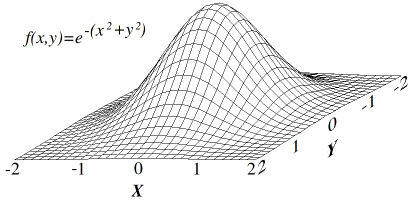
\includegraphics[width=0.6\textwidth,scale=1]{files/Hill_climb.png}  
		\caption{A convex function. Ideal for the hillclimbing method \cite{wiki-hill}.}
		\label{fig:hill}
	\end{figure}
\end{center}

\begin{center}
	\begin{figure}[H]
		\centering
		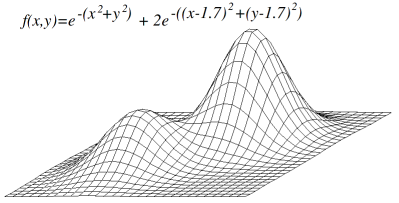
\includegraphics[width=0.6\textwidth,scale=1]{files/Local_maximum.png}  
		\caption{A function with two optima. Hillclimbing could end in the worse optimum if it starts at a bad coordinate. \cite{wiki-hill}.}
		\label{fig:hill2}
	\end{figure}
\end{center}


\section{Variants of the creepy random search method}
In the main-method of the creepy random search you just accept better fitness values after an iteration-step and reject worse ones.
The problem is, that with this algorithm you will mostly get stuck on a local optimum, instead of finding the global one.
To solve this problem you should allow temporal low fitness-values. It should be possible to leave a local optimum to find a better one.
To realise this, there have been developed some extended versions of this method: \\

\fbox{
	\begin{minipage}{15cm}
		\begin{itemize} 
			\item A stagnation of the fitness is allowed by a specified probability (Simulated annealing)
			\item A stagnation of the fitness is allowed untill a maximal deterioration. (Threshold accepting, deluge method)
		\end{itemize}
	\end{minipage}
} \\


\subsection{Simulated annealing}
Simulated annealing is a probabilistic optimization method.
It is inspired by the annealing of fluid materia to a solid aggregate states in metallurgy. While cooling down a material the thermodynamic free energy has to get as minimal as possible to get a clear crystalline structure. Therefore its suggested to cool down to material slowly for a better probability of getting a clear solid body.

Analog in optimization you start with a high temperature T, means reaching a wide area in the search space. That way it's possible to reach more maxima. At the beginning each chromosome has the same probability to get selected. With each iteration the temperature is reduced and the reached area is getting smaller. Selecting better chromosomes is now more probalistic.
Towards the end the algorithm commutes in an optimum and behaves like the standard hillclimbing-algorithm.

Slowly reducing the temperature increases the chance to find the global optimum. Cooling to fast leads to commuting early into a local optimum instead.

The following formula shows the probability of selecting a chromosome with lower fitness:

\begin{equation}
p(r) = \frac{1}{1+exp(-r/T)}
\end{equation} 

The probability to select a worse chromosome should be small.
At the beginning a big T tends to equalize the probability of all chromosomes. For $T \to \infty$ all chromosomes have the same chance to get selected. Lowering T gives good chromosomes priority.


\section{Crossover}
The crossover algorithm represents the idea of cultivating a population of individual solutions. After rating the population, the best individual is choosen and crossed with a random one of the actual population. There are two children created, who can optionally be mutated. This is done until the a new generation of individuals is created.
The process is repeated until a satisfying solution is cultivated or the process is aborted.\footnote{For more information see project work of Jonathan Schwarz}

\section{Applications}
The use of a specific algorithm depends on the problem and its modelisation. In general all optimization-methods are equal in effectivness, if we look over all posible optimization-problems in one set (No-free-Lunch-Theorem Source). Astonishingly a purely random search isn't less effective.
Some of the given methods are better in special cases than others. Also a good understanding of the problem's topic is essentially. Evolutinary algortihms take advantage of reducing the set of problems and a good modelisation.
Simulated annealing is suitable for functions with many local optima.



\chapter{The Box2D-Physicsengine}
Box2D is a 2-dimensional physics engine, created by Erin Catto. It is licensed under the zlib-license, hence it is noncommercial and open source. The Box2D library is written platform-independently in C++. It is used mainly for game development. Many portations into other programming languages, like Java and C\# exists. \\
(source jbox2d)


Box2D is used by the project to simulate a realistic physical environment, proving the agents behaviour. \\

Erin Catto wrote a testing gui, called Testbed, using the opengl-framework GLUT, respectively freeglut for windows.

The project-structure is based on the testbed-program.


\section{Core concepts}

\subsection{Bodies}
Bodies are the main objects, affected by physics-simulation.

A body contains the following values: \\

\fbox{
	\begin{minipage}{15cm}
		\begin{multicols}{2}
			\begin{itemize}
			\item \textbf{2D position vector}
			\item \textbf{Angle}
			\item \textbf{Velocity}
			\item \textbf{Angular velocity}
			\item \textbf{rotational inertia}
			\item \textbf{mass}
			\item \textbf{1 or more fixtures}
			\end{itemize}
		\end{multicols}
	\end{minipage}
}   \\
\\



A body contains one or more fixtures, containing the shape and more properties of the body.

If a body is moved, the fixtures are also moved.

\subsubsection*{Bodydefinitions}
To create a body, a bodydefinition has to be created first. It's holding the bodytype, linear- and angular damping values, among other things.
The bodydefinition can also be used to set the start- position and angle of the body. This can increase start-up performance.

\subsubsection*{Body types}
There are three types of bodies:

\fbox{
	\begin{minipage}{15cm}
		\begin{itemize} 
			\item \textbf{Static body}
			\item \textbf{Kinematic body}
			\item \textbf{Dynamic body}
		\end{itemize}
	\end{minipage}
}   \\
\\

A \textbf{static body} is excluded from the simulation. It also doesn't move. Static bodies are used as world-borders for example. Static bodies doesn't collide with other static- or kinematic bodies. \\

A \textbf{kinematic body} can move by setting its velocity, but isn't influenced by forces.
Kinematic bodies doesn't collide with other static- or kinematic bodies.\\

The \textbf{dynamic body} is the commonly used bodytype in Box2D-simulations. It is fully simulated and can be moved by the user or by forces, as its usual way.

\subsubsection*{Damping, friction and gravity scale}
\textbf{Damping} reduces the velocity (linear and angular) of the body.
\textbf{Friction} reduces the velocity of a body at collision with other bodies.

The damping parameter can be zero for no damping and infinite for full damping. In general a value between 0 and 0.1 is used.

The \textbf{gravity scale} is a factor that determines how much the worlds gravity influences the body. 0 determines no influence. The standard value is 1.

\subsubsection*{Activation and Sleeping}
A body can be set asleep. This is used to save cpu-time as for sleeping bodies there is no computing of physics necessary. The body will be woken up, if an other body collides with it.
A body can be completely excluded from simulation by setting it inactive instead.
In contrast to the sleeping-mode it will not be woken up.

%\subsubsection*{Methods}
%TODO

%\begin{lstlisting}[caption={Setting body definitions},label=lst:bodydef]
%b2BodyDef myBodyDef;
%myBodyDef.type = b2_dynamicBody;
%myBodyDef.position.Set(0, 20); //set start position
%myBodyDef.angle = 0; //set start angle
%\end{lstlisting}


%Transforming a body
%Set Velocity
%Set Angular velocity

\subsection{Fixtures}
Fixtures give bodies a shape and additional properties. A body can have multiple fixtures, with their positions relativly to the body's origin.

The following properties are part of a fixture:


\fbox{
	\begin{minipage}{15cm}
	\begin{multicols}{2}
		\begin{itemize} 
			\item \textbf{A shape}
			\item \textbf{Broad-phase proxies}
			\item \textbf{Density}
			\item \textbf{Friction}
			\item \textbf{Restitution}
			\item \textbf{Collision filtering flags}
			\item \textbf{Pointer to the affiliated body}
			\item \textbf{User data}
			\item \textbf{Sensor flag}
		\end{itemize}
	  \end{multicols}
	\end{minipage}
}   \\
\\

A single \textbf{shape} is contained by the fixture. The shape can be a rect, a polygon or a circle. Shapes aren't linked to the body directly, because they may be used independly of the simulation. Therefore the fixture is interposed between body and shape. In Box2D the maximum amount of vertices is defaultly set to eight. A vertex defines the position-vector of a body's edge. A polygon therefore can be created with a minimum of three position-vectors and maximally with eight.
\\

\textbf{Broad-phase proxies} are used internally by Box2D to accelerate collision detection. Therefore a dynamic tree containing the collision-pairs in form of AABB's\footnote{AABB: Axis aligned boundary box. AABBs are used for fast computing of collision detection} are used. In the most cases it isn't necessary for the user to use proxies. \\

The \textbf{densitiy} is used for computation of the body's mass.\\

The \textbf{friction} of two fixtures is multiplied at collision. \\

\textbf{Restitution} makes a fixture elastic. Usually this value is set between 0 und 1. \\

\textbf{Collision filtering flags} can be used to just allow specified groups of fixtures to collide. \\

A \textbf{pointer to the affiliated body} is stored in the fixture.\\

\textbf{User data} is used as a 'hook' to identify a fixture by an id or add it some self-defined properties. User data is a 'void *'-pointer. Therefore it can contain any datatype. \\

The \textbf{sensor flag} defines that a fixture doesn't interact physically with other fixtures, except by detecting collisions. \\



A fixture is created by initializing a fixture definition and passing its address to the body:

\begin{lstlisting}[caption={Creation of a fixture (source Box2D manual)},label=lst:fixture-create]
b2FixtureDef fixtureDef;
fixtureDef.shape = &myShape;
fixtureDef.density = 1.0f;
b2Fixture* myFixture = myBody->CreateFixture(&fixtureDef);
\end{lstlisting}


\subsection{Joints}
Joints are used to connect two or more bodies. For more detailed information read the Box2D manual Chapter 8.

\subsection{World}
A world is the simulation-environment. It contains all bodies and joints and manages all aspects for simulation. It is the main entity.

The world represents a factory pattern, because it can create and detroy bodies and joints.

\subsubsection*{Simulation parameters}
The physics-simulation is controlled by three parameters: \\

\fbox{
	\begin{minipage}{15cm}
		\begin{itemize} 
			\item \textbf{timeStep} (float32) (Recommended: 1.0f /60.0f respectively 60Hz)
			\item \textbf{velocityIterations} (int32) (Recommended: 8)
			\item \textbf{positionIterations} (int32) (Recommended: 3)
		\end{itemize}
	\end{minipage}
}   \\
\\

These parameters are used by the step-method of the world in which one single simulation step is processed. \\

The \textbf{timeStep} parameter defines the time-resolution on which the simulation will update the environment. A lower timestep improves the quality of the simulation, but on costs of performance. A higher timestep increases the performance, but the simulation can be inaccurate on too low values.
The default value is 60Hz. The author of Box2D suggests not to use values lower than 30Hz. As set, the timestep should not be changed as it could cause unwanted behaviour. For a faster simulation the step-method should just called multiple times. \\


\textbf{Velocityiterations} is the resolution of computing impulses to move bodies precisly. The default value is 8. \\

\textbf{Positioniterations} defines the resolution of overlapping bodies. This is important for a correct collision detection of bodies. The default value is 3. \\


source: www.iforce2d.net/b2dtut/worlds
source: box2d.org/manual.pdf

\subsubsection*{Methods}
TODO
\begin{lstlisting}[caption={World creates a body},label=lst:world-body]
b2Body* m_body = m_world->CreateBody(&myBodyDef);
\end{lstlisting}

\section{Collision detection}
In Box2D collisions are computed between two fixtures. A contact object, containing information about collision coordinates, normals and impulse among ohter things, is created if a collision happens. A contact object can be used to manage a collision.

An AABB is an 'axis aligned bounding box'. It completly contains a shape. It is used for fast performance of computing geometrical operations. (source: wikipedia)

\begin{center}
	\begin{figure}[H]
		\centering
		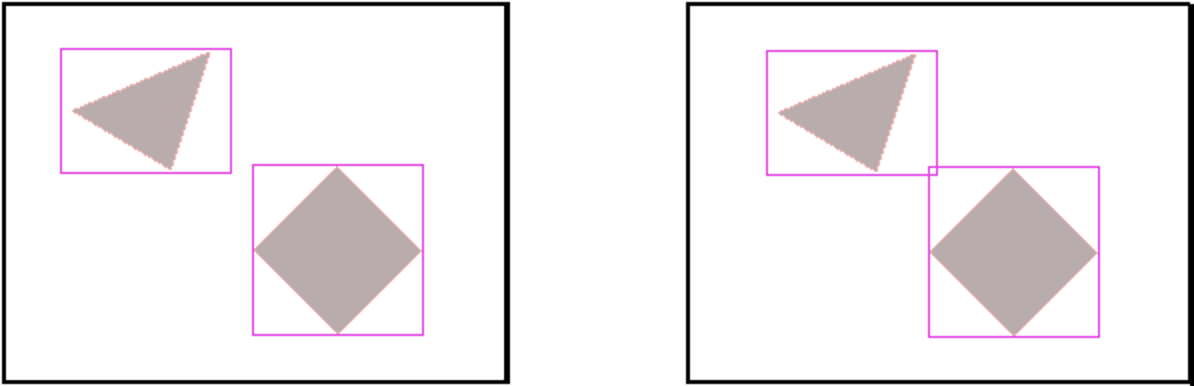
\includegraphics[width=0.8\textwidth,scale=1.0]{files/aabbs-crossing.png}  
		\caption{Two AABBs are overlapping. (source iForce2D) \cite{box2d-iforce}.}
		\label{fig:aabbs}
	\end{figure}
\end{center}
If two AABBs are overlapping, a contact between the two fixtures is created, but the isTouching()-method returns 'False', because the shapes aren't overlapping.

Sometimes, fast moving bodies misses collisions. Therefore it is possible to define the body as a bullet for high resolution at collisions, in cost of performance.
This can be accomplished at creation of the body, by the body's definition instance:

\begin{lstlisting}[caption={Define fixture as bullet before creation},label=lst:fixture-bullet-before]
bodyDef.bullet = true;
\end{lstlisting}

Or after the creation of a body by the following method:

\begin{lstlisting}[caption={Define fixture as bullet after creation},label=lst:fixture-bullet-after]
body->SetBullet(true);
\end{lstlisting}

The following figure shows the processing of a collision:

\begin{center}
	\begin{figure}[H]
		\centering
		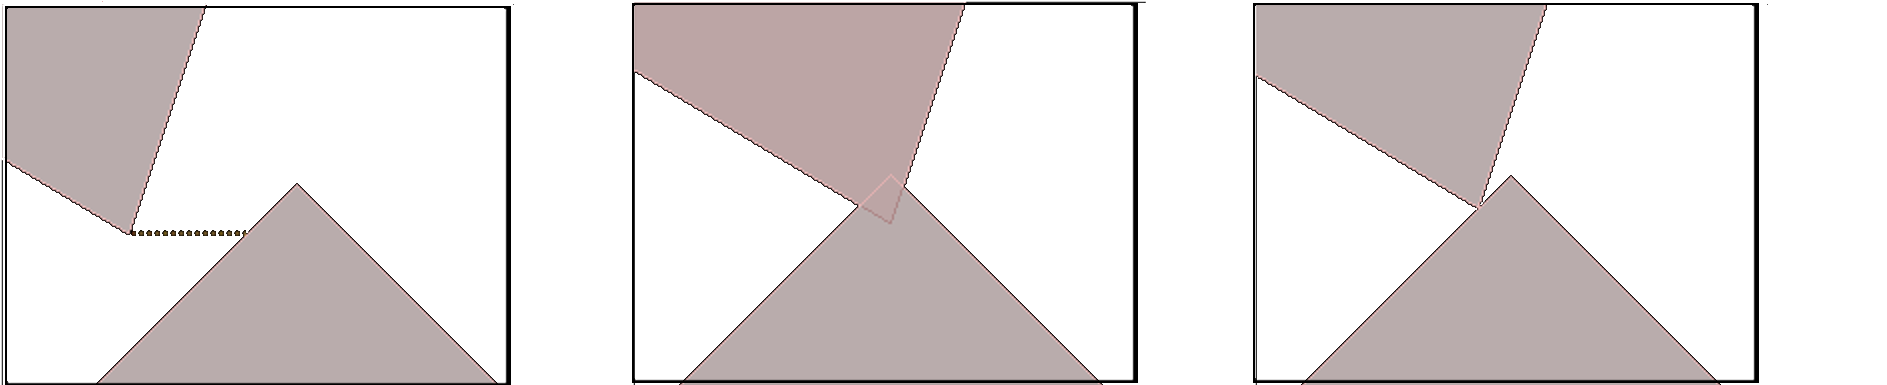
\includegraphics[width=1.0\textwidth,scale=1.0]{files/fixtures-overlap.png}
		\caption{Two fixtures are overlapping (source iForce2D) \cite{box2d-iforce}.}
		\label{fig:fixture-overlap}
	\end{figure}
\end{center}

In the first picture, a contact is created, because the AABBs of the two object are overlapping.
The second picture shows non-bullet bodies overlapping. A bullet-body takes more cpu-time to compute but would get picture three as result.

Bullet bodies

\subsection{Contact listener}
The contact listener executes callback-methods if the events 'Begin contact' or 'End contact' are triggered.
On a collision a contact object is created containing information about the fixtures collision.
Contacts are used to manage collisions between two fixtures.

To access the contact and the two colliding fixture a contact listener should be used.

The collision-computation processes four phases: \\

\fbox{
	\begin{minipage}{15cm}
		\begin{itemize} 
			\item \textbf{Begin contact}
			\item \textbf{Presolve} 
			\item \textbf{Postsolve}
			\item \textbf{End contact}

		\end{itemize}
	\end{minipage}
}   \\
\\


source: iforce2D


\begin{lstlisting}[caption={Contact listener methods},label=lst:collision-contact]
/b2ContactListener
// Called when two fixtures begin to touch
virtual void BeginContact(b2Contact* contact);
// Called when two fixtures cease to touch
virtual void EndContact(b2Contact* contact);
// Called after collision is detected
virtual void PreSolve(b2Contact* contact, const b2Manifold* oldManifold);
// Called after computing the results of the collision
virtual void PostSolve(b2Contact* contact, const b2ContactImpulse* impulse);
\end{lstlisting}

\subsubsection*{Begin contact}
This callback is executed when two fixtures begin touching.

\subsubsection*{End contact}
The end contact callback is called when the two colliding fixtures cease touching.

\subsubsection*{Presolve}
The presolve callback is executed after detection of a collision, but before computing the resulting impulses. It contains a pointer to the contact.

\subsubsection*{Postsolve}
The postsolve callback is executed after computation and applying the contactimpulses of the collision. It contains a pointer to the contact and also the computed impulsedata.

\subsection{Collision filtering}
The default behaviour is that all fixtures can collide with each other. If you want to specify which groups of fixtures can collide and which pass through each other, you can use category- and mask bits to manage 16 groups of fixtures. If you need more precise behaviour you can use group indizes or define own rules by overriding the 'ShouldCollide'-method.

\subsubsection*{Category- and maskbits}

These bits are 16-Bit wide and therefore 16 groups are supported.
Category bits declare on which groups a fixture belongs. A fixture has to belong to minimal one and maximal 16 groups.
The mask bit defines the group of fixtures this fixture can collide with. The default values are 0x0001 for category bits and 0xFFFF for mask bits, meaning every fixture can collide with each other.

\subsubsection*{Group indizes}
Group indizes can be used to get a more specified behaviour as only with category- and maskbits.
The standard value of the group index for a fixture is zero, means group index isn't used, instead the category- and maskbits are used. The value otherwise can be positive or negative.

For a value nonzero the following rules are applied at collision: \\

\fbox{
	\begin{minipage}{15cm}
		\begin{itemize} 
			\item if both groupindizes are different, use the category/mask rules as described above
			\item if both groupindizes are equal and positive, collide
			\item if both groupindizes are equal and negative, don't collide
		\end{itemize}
	\end{minipage}
}   \\
\\

\subsubsection*{Contact filter}
For an userdefined specification of collision behaviour the following virtual method can be overwritten: \\
\begin{lstlisting}[caption={The contact filter method},label=lst:box2d-contactfiler]
bool b2ContactFilter::ShouldCollide(b2Fixture* fixtureA, b2Fixture* fixtureB);
\end{lstlisting}


\section{DebugDraw}
The debugdraw class is used as a debugging feature to display the physics simulation of Box2D. It uses OpenGL. Debugdraw can draw the shapes, contact points, contact normals, the AABBs, etc.
As the debugdraw offers all wanted basic shapes it is used by the simulator.

To use the debug-draw first the debugdraw object hast to be instanciated and linked to the world by: \\

\begin{lstlisting}[caption={Linking debugdraw instance to the world instance},label=lst:box2d-ddrawset]
m_world->setDebugDraw(&m_debugDraw);
\end{lstlisting}

Setting the flags to determine what has to be drawn:

\begin{lstlisting}[caption={Initializing DebugDraw},label=lst:box2d-ddrawinit]
uint32 flags = 0;

flags += b2Draw::e_shapeBit; //Enable drawing shapes
flags += b2Draw::e_jointBit; //Enable drawing joints
flags += b2Draw::e_aabbBit; //Enable drawing AABBs
flags += b2Draw::e_centerOfMassBit; //Enable drawing center of masses

m_debugDraw.SetFlags(flags);
\end{lstlisting}


After each calling of the step-method the following method has to be called: \\

\begin{lstlisting}[caption={Using debugdraw after each step},label=lst:box2d-ddraw]
m_world->DrawDebugData();
\end{lstlisting}

This draws every shape in the bodylist of the world.
 \newpage
\section{Structure of a Box2D-Project}
As follows, you can see the general structure of a Box2D-Project: \\

\begin{center}
	\begin{figure}[H]
		\centering
		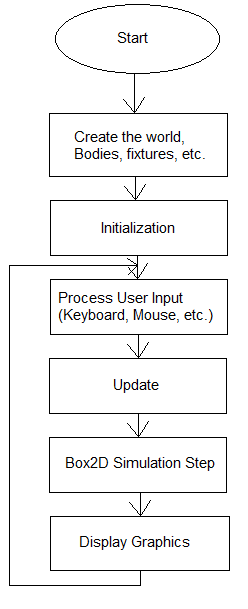
\includegraphics[width=0.4\textwidth,scale=0.5]{files/Box2D-Structure.png}
		\caption{The general structure of a Box2D-application} \cite{box2d-structure}
		\label{fig:box2d-structure}
	\end{figure}
\end{center}

TODO: short description

%Important: In BeginContact and EndContact no change of active-flag and some other values of a body/fixture


\section{Testbed}

TODO

%AnimalFixtureDef[i].isSensor = false;
%AnimalFixtureDef[i].friction = 1.0f;
%AnimalBodydef[i].linearDamping = 1.0f;
%AnimalBodydef[i].angularDamping = 2.0f;

\chapter{The OpenGL graphics library}
OpenGL stands for Open Graphics Library. It is a widely used for developing graphics applications and was published in 1992 by Silicon Graphics. Since 2006 it is maintained by the Khronos Group. It is licensed under a open source license. The logo and the trademark are licensed under a trademark-license.
OpenGL is platform-independent.


It is used by the project to accelerrate the simulator.

The Box2D-Testbed uses GLUT respectively Freeglut and GLUI. Thererefore theses libraries are also used in this project.

source: www.opengl.org
www.sgi.com/tech/opengl/?/


\section{The OpenGL Utility Toolkit (GLUT)}
The OpenGL Utility Toolkit (GLUT) was developed by Mark Kilgard. It is used to extend OpenGL-Applications by window-management. GLUT is used for small- and medium sized OpenGL-applications.

source: www.codeproject.com/Articles/19760/GLUT-Window-Template

www.opengl.org/resources/libraries/glut/

\subsection{Freeglut}
Freeglut is developed by Pawel W. Olszta and is an alternative to GLUT. It is also a Windows substitute. Freeglut is still maintained. Freeglut is used, because the originally GLUT-library is deprecated and not maintained anymore.

source: freeglut.sourceforge.net/

\subsection{Program structure}
In this section the basic structure of a freeglut-program is explained.
The following code shows the initialization and creation of a window:

\begin{lstlisting}[caption={Initialization a GLUT-program},label=lst:glut-init]
#include "glut.h"

int mainWindow;  //Window handler

int main(int argc, char* argv[])
{
  // Glut initialitation
  glutInit(&argc, argv);
  glutInitDisplayMode(GLUT_RGBA | GLUT_DOUBLE);
  glutInitWindowPosition(0, 0); 
  glutInitWindowSize(1024, 768);
  
  mainWindow = glutCreateWindow("Title");
  
  //Register function callbacks
  glutDisplayFunc(Display);
  glutKeyboardFunc(Keyhandler);
  glutReshapeFunc(Resizehandler);
  
  //Here optionally a GLUI-window can be included, see Chapter 6.3
  
  //Enter glut main loop, usually no return from this function
  glutMainLoop(); 
  return 0;
}
\end{lstlisting}

In the first lines glut is initialised, a window with specified position, size and a title is created.
The variable 'mainWindow' is of type int. It stores the adress of the window-structure.

In the second part of the codesnippet the handler-functions are set. The handler functions have to be static functions.
At the end the glut main loop is entered. Usually this function never returns. In Freeglut there exist functions to leave and re-enter the main loop.

The following Codesnippet shows the drawing of a simple triangle:

\begin{lstlisting}[caption={Drawing some graphics},label=lst:glut-draw]
static void Display()
{
  //Set the color to white
  glClearColor(0.0f, 0.0f, 0.0f, 1.0f);
  //Clear the Scene with selected color
  glClear(GL_COLOR_BUFFER_BIT | GL_DEPTH_BUFFER_BIT);
  //Switch to Modelview Matrix
  glMatrixMode(GL_MODELVIEW);
  //Replace the current matrix by the identity matrix
  glLoadIdentity();
  //Draw a blue triangle into the buffer
  glColor3f(0.0f, 0.0f, 1.0f);
  glBegin(GL_TRIANGLES);
  glVertex3f(-0.5f, 0.5f, -5.0f);
  glVertex3f(-1.0f, 1.5f, -5.0f);
  glVertex3f(-1.5f, 0.5f, -5.0f);
  glEnd();
  //Finally draw the scene on screen
  glutSwapBuffers();
}
\end{lstlisting}

The first line sets the draw-color to white and with no transparency. The color is formatted in RGBA. The first three parameters represent the colors red, green and blue. The last parameter is alpha, the transparency of the figure. 0.0f means no quantity of the according parameter and 1.0f as the full quantity.
 This is used by the second line to clear the scene.
Then the viewmode is set, the position of the camera is loaded.
With 'glBegin' the drawing of an object is started. In this example a triangle is drawn. Therefore the three vertices of the triangle has to OpenGl. This is done by. Each object has to finished with the 'glEnd'-command.
At the end the buffer is swapped and the drawn scene is displayed at the screen.

\begin{lstlisting}[caption={Resize camera perspective on window resize},label=lst:glut-resize]
static void Resize(int w, int h)
{
//Set the viewport of the camera
glViewport(0, 0, w, h);
//Switch to the camera perspective matrix
glMatrixMode(GL_PROJECTION); 
//Reset the camera matrix
glLoadIdentity();
//Set camera angle, width-to-height ratio, near z and far z clipping coordinate
gluPerspective(45.0f, (double)w / (double)h, 1.0f, 200.0f);
}
\end{lstlisting}

The first line sets the viewports position and size. The following operations should than applied on the projection-matrix. Therefore the Matrix is resetted to the identity matrix and the clipping of the world the camera should record is set. The near z-coordinate sets the 2D-viewing plane of the camera. The 3D-world will be projected on this 2D-plane. This is the picture that the user will finally see. The far-z perspective defines how deep the sight of the camera into the world is. Objects out of range aren't considered in this case. \\

TODO: Figure of the camera perspective

\section{The OpenGL User Interface Library(GLUI)}
The OpenGL User Inteface Library (GLUI) is a GLUT-based user interface library developed by Paul Rademacher. It is written in C++ and usable for multiple platforms.

GLUI is used to implement GUI controls, like buttons, labels, listboxes, etc.

The following figure shows some components of GLUI:

\begin{center}
	\begin{figure}[H]
		\centering
		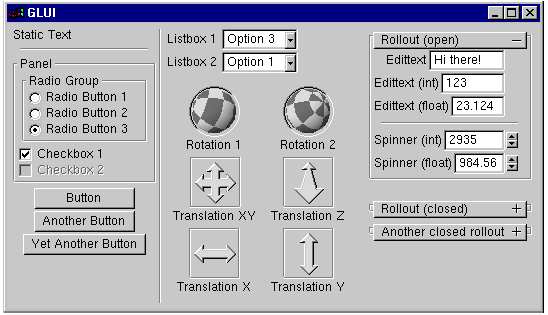
\includegraphics[width=0.8\textwidth,scale=1.0]{files/glui.png}  
		\caption{Some GLUI Components (source www.cs.unc.edu/~rademach/glui/) \cite{ogl-glui}.}
		\label{fig:ogl-glui}
	\end{figure}
\end{center}

source: www.codeproject.com/Articles/20286/GLUI-Window-Template

glui.sourceforge.net/


\subsection{GLUI-Program}
In this section is described how a GLUI-window is set up.
The following code is included after the creation of a GLUT-window and before entering the glut main loop (see \ref{lst:glut-init}) :


\begin{lstlisting}[caption={Creating a GLUI-window},label=lst:glui-create]
#include "glui.h"
//GLUI window instance
GLUI *glui;

int main(int argc, char* argv[])
{
 ...
 //after creation of glut-window
 glui = GLUI_Master.create_glui("GLUI", 0);
 //Add some components
 glui->add_statictext( "Simple GLUI Example" );
 glui->add_separator();
 glui->add_checkbox( "Wireframe", &wireframe, 1, control_cb );
 GLUI_Spinner *segment_spinner =
 glui->add_spinner( "Segments:",GLUI_SPINNER_INT, &segments );
 segment_spinner->set_int_limits( 3, 60, GLUI_LIMIT_WRAP );
 GLUI_EditText *edittext =
 glui->add_edittext( "Text:", GLUI_EDITTEXT_TEXT, text );
 //Set the main gfx window
 glui->set_main_gfx_window(main_window);
 //Register the Idle callback with GLUI (instead of with GLUT)
 GLUI_Master.set_glutIdleFunc(GlutIdle);
}
\end{lstlisting}

First the glui-instance is initialized. In the following lines gui-components are added. Some components need a variable to point on. This is necessary to store input values from the user. The components can be dimensionized, e.g. the spinners minimum and maximum value is set.
At the end the corrosponding glut window has to be registered in the glui-window.
Callbacks are now defined. This has to be static functions, like in GLUT.

'GLUI\_Master' is a global GLUI-object used to register callbacks, as glui-windows use for example the idle-callback extensively to control components status.

\chapter{Implementation}

\section{Concept}
The main concept is to cultivate a population of agents by different evolutionary algorithms to find a satisfying solution. Each agent has a sensor, representing an own coordinate system. The agents have to collect as much objects as possible within a given time. Therefore it has a feedforward neural network realized as multilayer perceptron.
The objects and the agents are spawned randomly every round.

\begin{center}
	\begin{figure}[H]
		\centering
		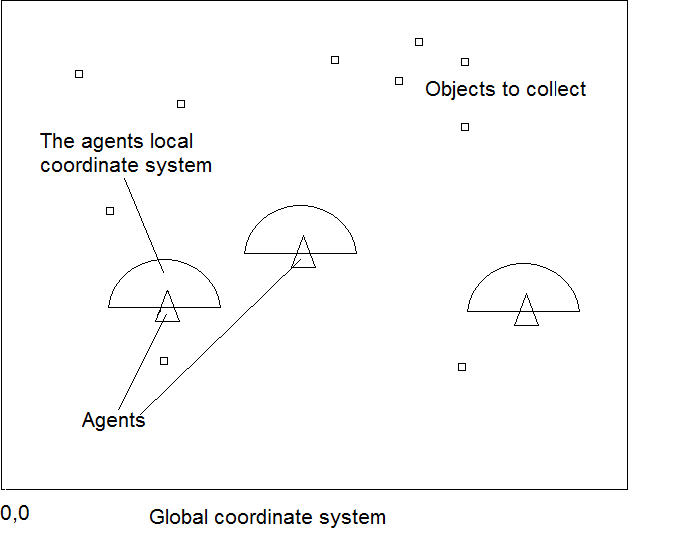
\includegraphics[width=0.7\textwidth,scale=1.0]{files/main-concept.png}  
		\caption{A sketch of the main concept}
		\label{fig:concept-main}
	\end{figure}
\end{center}

\subsection{The task environment}
The simulation environment is: \\

\fbox{
	\begin{minipage}{15cm}				\begin{multicols}{2}
		\begin{itemize} 
			\item \textbf{partially observeable}
			\item \textbf{single agent based or mulitagend based and competive} 
			\item \textbf{deterministic}
			\item \textbf{episodic}
		    \item \textbf{static}
		    \item \textbf{continous}
		    \item \textbf{known}, because the sensors give all necessary values
		\end{itemize}
	\end{multicols}
	\end{minipage}
}   \\
\\

The simulation environment is \textbf{partially observeable} because the agents perception is limited by the sensor that has a fixed radius. \\

It can be both \textbf{single agent based or mulitagend based and competive}, depending on the population size. If there is just one agent to train its single agent based, with more agents multiagent based and competive. \\

The environment is \textbf{deterministic}. The start positions are choosen randomly, but the process of collecting the objects is from this point on deterministic as each step to get objects can be desribed step by step. \\

Its \textbf{episodic} as the actual state does not change the general method of collecting further objects.

The task environment is \textbf{static}, even if there are multiple agents we consider a static behaviour of the environment for simplicity. The agent don't interrupt each other to often. \\

\textbf{Continuity} is given, because we handle with real values like the acceleration, the rotation and real valued neuron weights. The time for one generation is also continous. \\

The environment is \textbf{known} as the agents sensor gives all data necessary to solve the task.\\

\subsection{Realizing the agent}
In this project work a simple reflex agent is realized.
The agents processing logic is realized by a multilayer perceptron. That means the agent has no memory and just processes the actual perception\footnote{To get a memory a recurrent neural network could be used}. This categorises the agent to a simple reflex agent.

\subsubsection*{The agents sensor}
The agents sensor is a semicircle detecting just collectable objects in an given radius. The sensor returns a vector containing the X- and Y-coordinate relative to the agents actual position.

\subsubsection*{The agents actuator}
The agent can rotate left or right.
The agent can accelerate just forwards.


\subsection{Coordinate system transformation}

To get the relative position of an object the global coordinate system has to be transformed into the agents local coordinate system, considering the agents actual angle.

Therefore at first a translation is made, then the rotation of the agent is applied.

\begin{center}
	\begin{figure}[H]
		\centering
		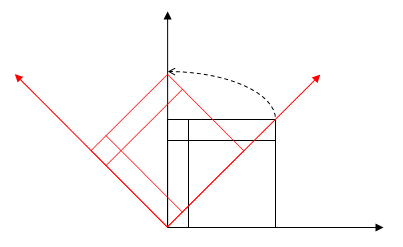
\includegraphics[width=0.5\textwidth,scale=1.0]{files/CoordinateRotation.png}  
		\caption{(Source https://de.wikipedia.org/wiki/Koordinatentransformation) \cite{wikipedia}.}
		\label{fig:cosys-transform}
	\end{figure}
\end{center}

\begin{equation}
\vec{P'}^{\,} =
\begin{pmatrix}
\cos \alpha & \sin \alpha & 0 \\
-\sin \alpha & \cos \alpha & 0 \\
0 & 0 & 1
\end{pmatrix}
* \vec{P}^{\,}
\end{equation}

\begin{equation}
x' = x * \cos \alpha + y * \sin \alpha
\end{equation}
\begin{equation}
y' = -x * \sin \alpha + y * \cos \alpha
\end{equation}

Source: Wikipedia


Transformation of the inputvalues through the input-neurons from range [-20.0, 20.0] and [0.0, 20.0] (Sensor x and y) and [-Pi, +Pi] (DeltaAngle) to the range [-1.0,+1.0] or [0.0, 1.0] with tanh function. (Better function? Linear function?)

Explain why DeltaAngle is necessary:
rotate clockwise. If Agent is rotated by 180degree error should rotate counter-clockwise,but
has learned to rotate clockwise without deltaangle as input.


Optional: Random placement of Objects and agents: see algorithm in NeuralWorld.cpp



Scalability of the World


Modes:
Singleplayer with recording
Supervised learning:
Evolutionary algorithms

Scalable World:
- Size
- Amount of Objects
- Amount of Agents

\section{The graphical user interface}


\begin{center}
	\begin{figure}[H]
		\centering
		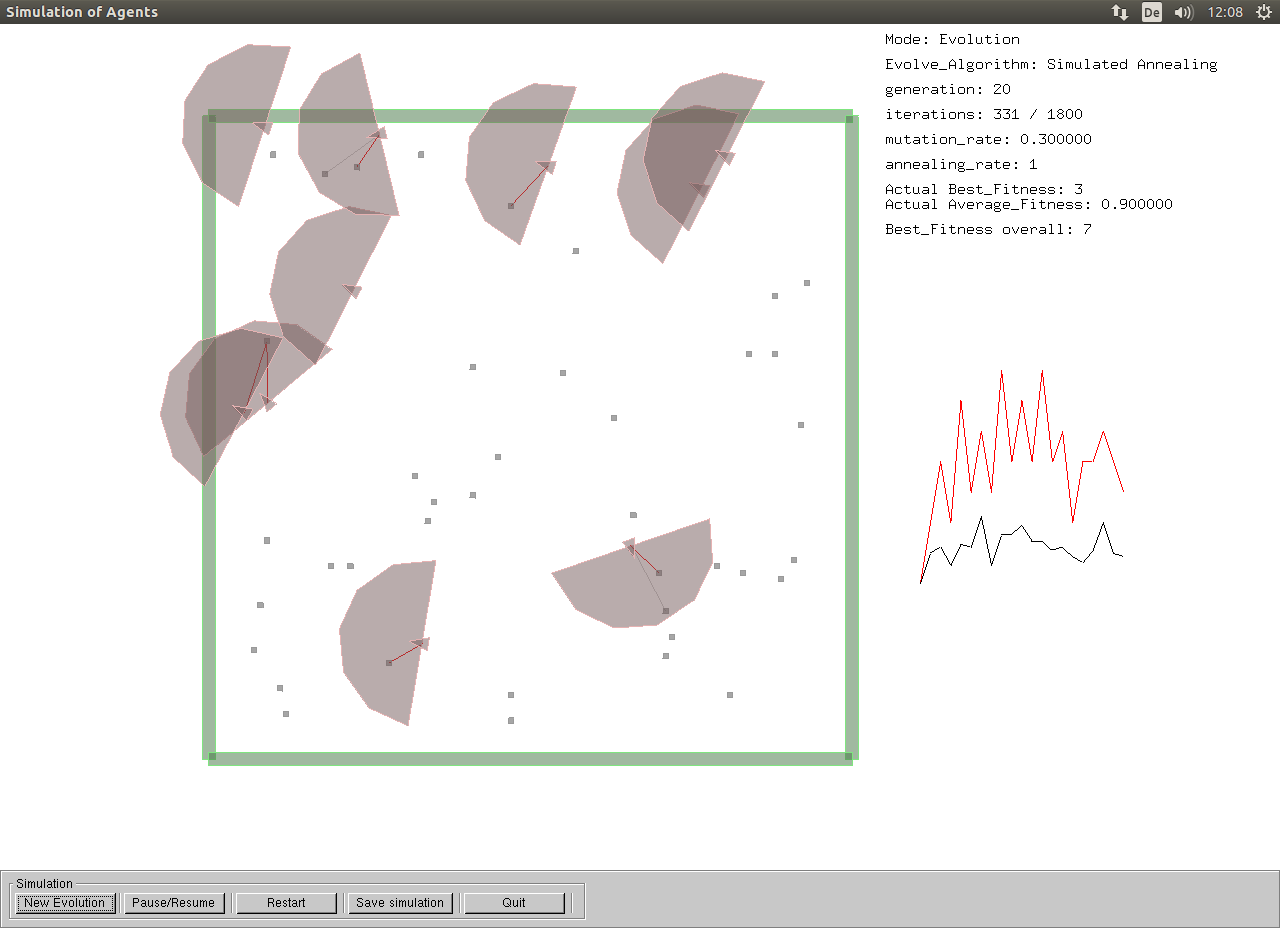
\includegraphics[width=1.0\textwidth,scale=1.0]{files/new_graphic.png}  
		\caption{new graphic}
		\label{fig:cosys-transform}
	\end{figure}
\end{center}


\begin{center}
	\begin{figure}[H]
		\centering
		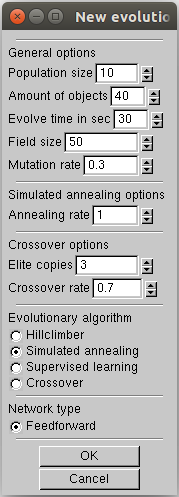
\includegraphics[width=0.2\textwidth,scale=1.0]{files/new_graphic_new_ev.png}
		\caption{new graphic create evolution}
		\label{fig:cosys-transform}
	\end{figure}
\end{center}



\subsection{Visualisation}

Fitness Graph
Weight Matrix
Neural Network
% \subsection{The fitness-function}


% \subsection{Neural networks}



\section{Software-Engineering}

\subsection{Classdiagram}

\subsection{Use-Cases}



Buttons, Modes

Optical Design of the gui

Weight-Matrix

Neural Network Activation


The inputs: 
x  [0.0, 20.0]
y   [0.0, 20.0]
alpha  [-PI, PI] (Radians)

If no object is detected :
x = 0
y = 0,
alpha = 0 

If an object is detected:
x= Agent.x - Object.x  
y = Agent.y - Object.y
alpha = Agent.Angle - (atan2(det, dot)) 
alpha is the difference between the actual direction of the agent and
the angle between the Position vector of the agent and the object. 
Helpervariables:
determinant: det =  Agent.x * Object.y - Agent.y * Object.x 
dot product:  dot =  Agent.x * Object.x + Agent.y * Object.y 


Outputs are:
Acceleration of the agent: [0.0, 1.0] (with a resolution of 0.001)
multiplied with the maximum accelartion of 
(-sin(Agent->GetAngle())*0.075f * 500 * ,  cos(Agent->GetAngle())*0.075f * 500)

Rotation by angle the agent: [-1.0, 1.0] (with a resolution of 0.001)
multiplied with the maximum rotationspeed of 0.075


\subsection{File saving and loading}

TODO Parser diagram loading the data.

%The
%To minimize  that the agents are missing

\section{OpenGL}
Used to accelerate the simulation.


GLUT, Windows Substitute Freeglut and GLUI. (used because Box2D Testbed used it)

\subsection{Rendering system}

\subsection{ViewPort}

\subsection{MainLoop}

Concept

\subsection{ViewPort}

\section{Box2D}

\subsection{The interface}
(to the concrete implementation in Box2D)


Call the Step-multiple times instead of changing the timestepvalue

Care that the fixture shapes center is at (0,0) (The body's center). Can be problem at rotation if shape is not centered.

Coordinate system transformation for each agent.

Sensor as semicircle (Source: iforce2D Radarsensor)

Detection of food: atan2-function

\section{Tools}
Make, CMake
Python for Trainingdata



\chapter{Results of the simulation}

\section{A simple script}
The simple script is based on trigonometric function.

\section{The hillclimber method}

\section{Simulated annealing}



\chapter{Conclusion}




\KOMAoptions{listof=leveldown}

\newpage

%=========================================LISTS=========================================

\listoffigures
\listoftables
\listofalgorithms
\lstlistoflistings

\newpage

%=========================================DICTIONARY====================================

%dictiary style
\bibliographystyle{./files/alphadin}
%dictionary source
\bibliography{./files/bibdb}


%AI-Junkie Smart Sweepers

%Evolutionäre Algorithmen
%Theorie der neuronalen Netze
%Jonathan Schwarz
%Künstliche Intelligenz

%Box2D Manual
%Box2D Iforce2D

%CMake Manual
%Makefile Manual

%Software-Engineering books?

%Opengl, GLUT and GLUI



\end{document}
